\begin{figure}[!htb]
     {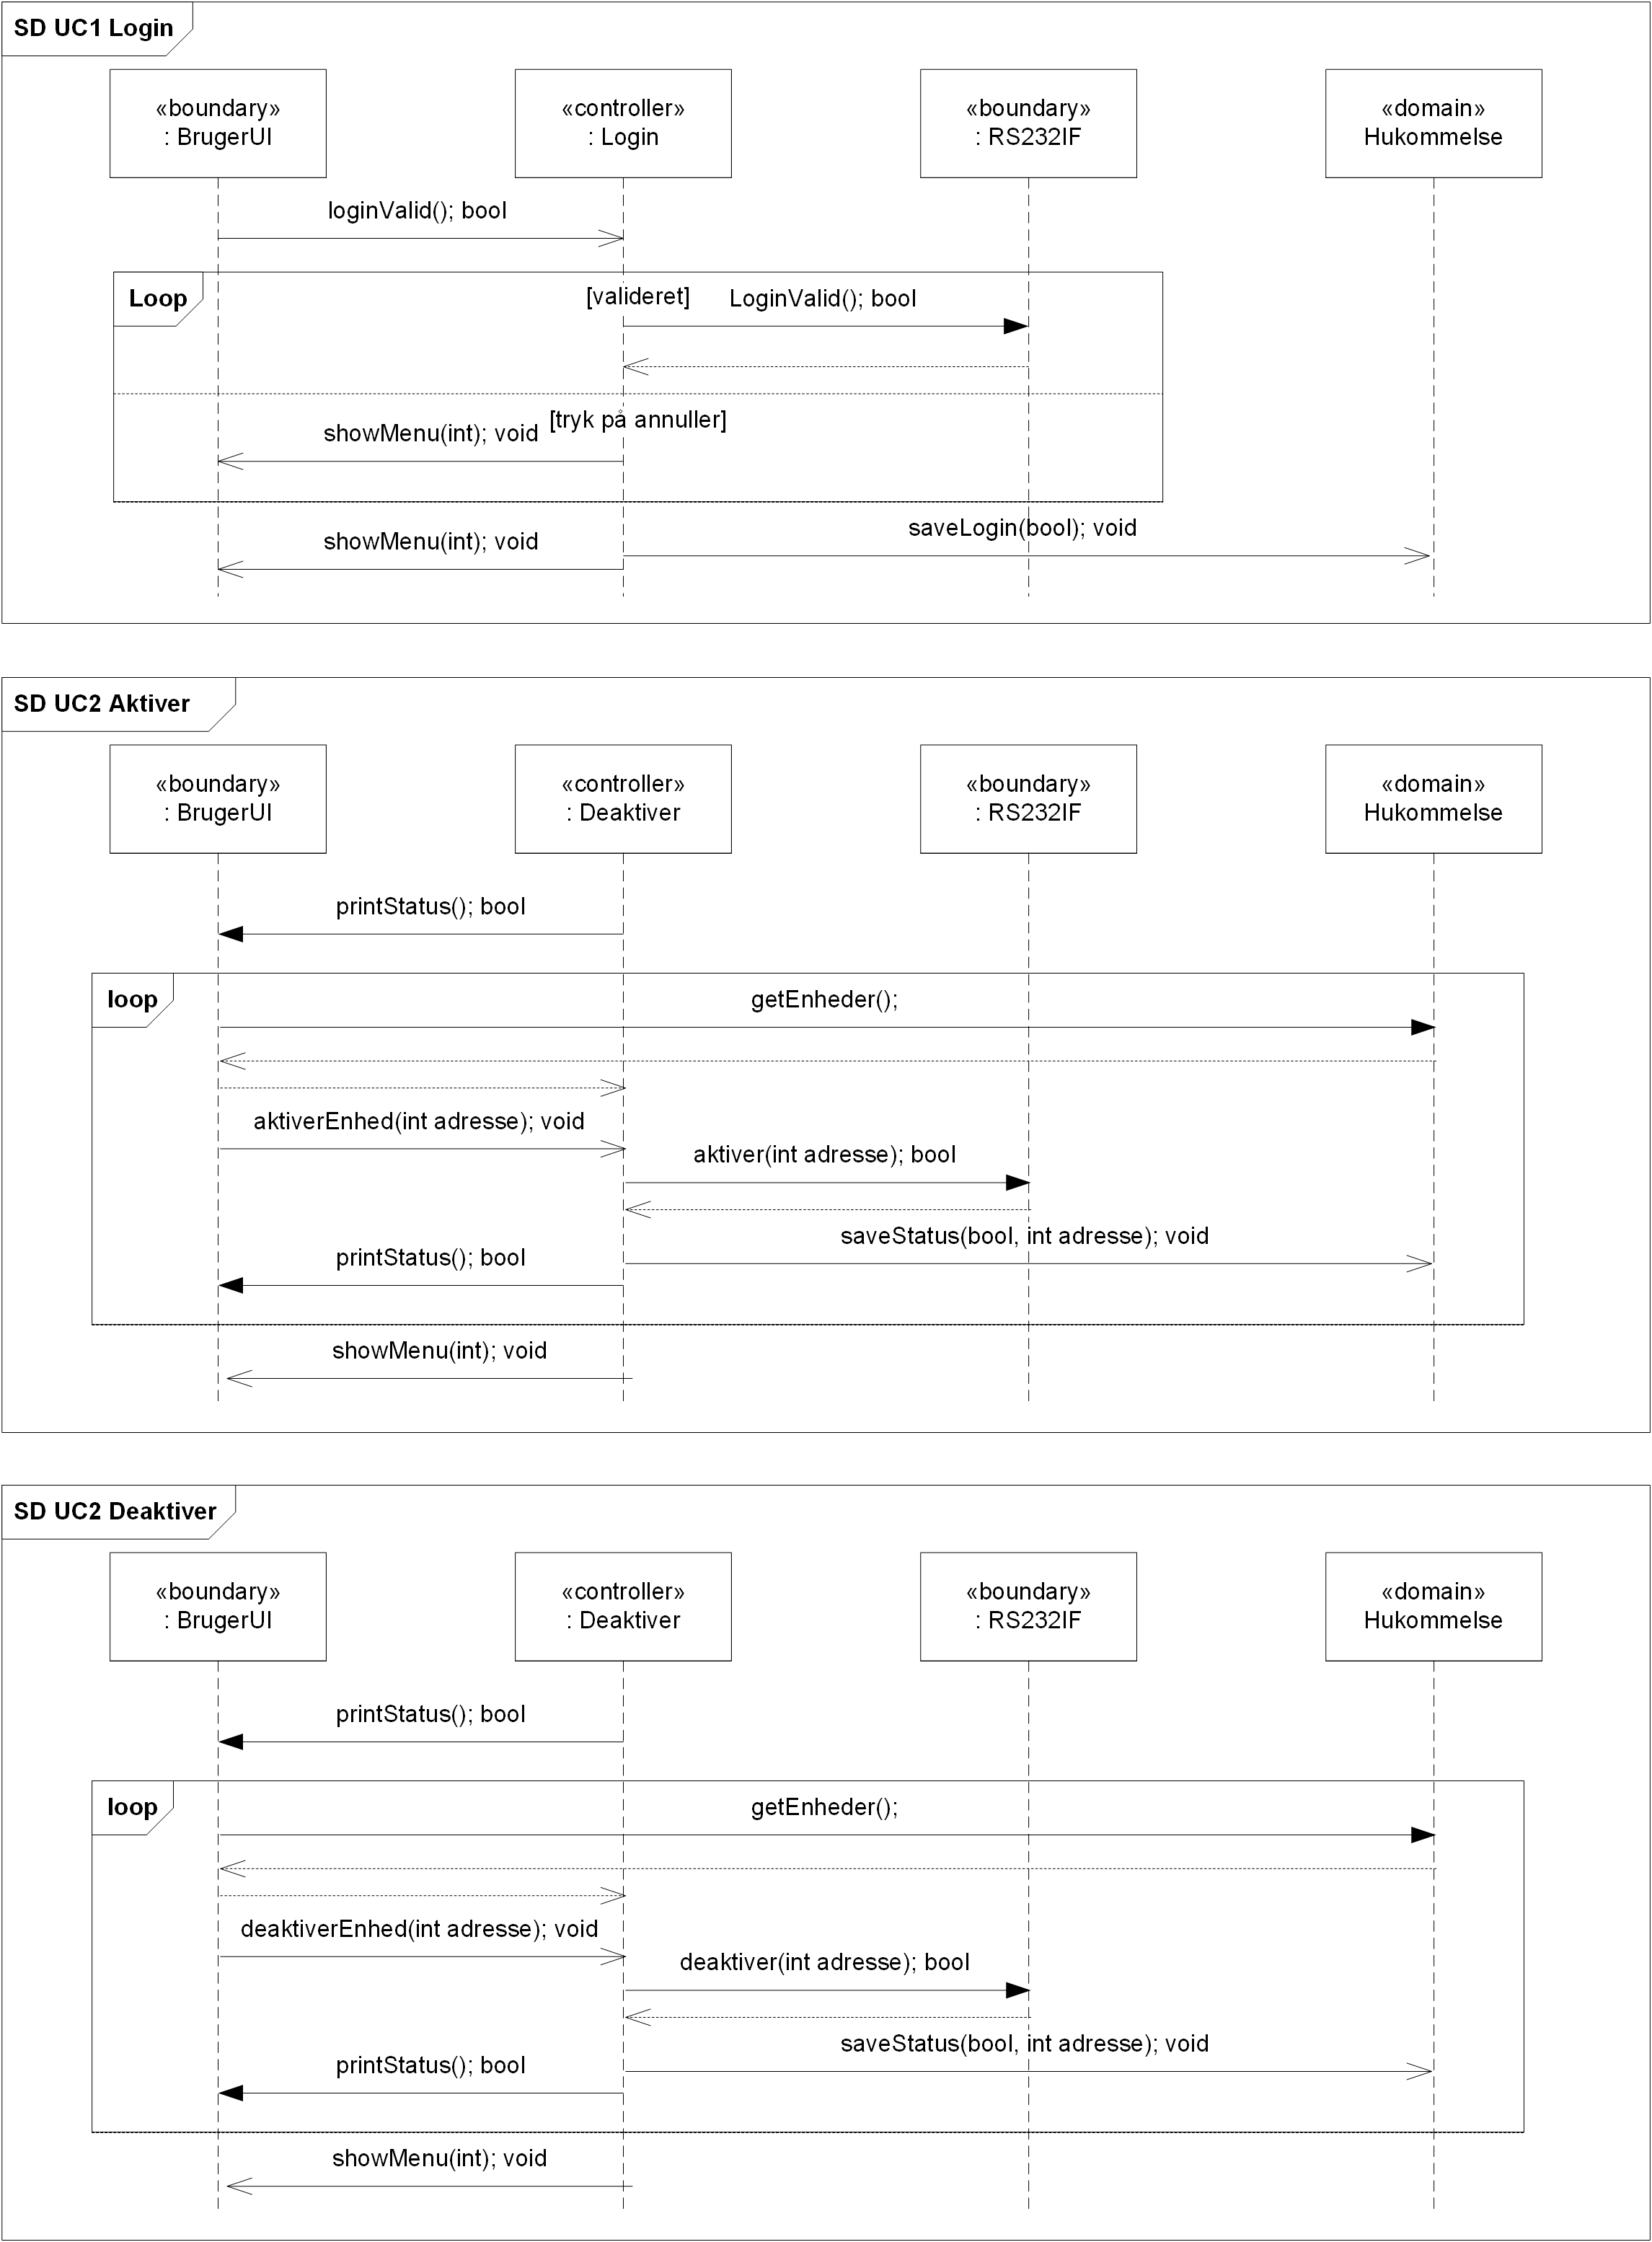
\includegraphics[width=\textwidth]{billeder/uml/PC_SD1}}
     \caption{Use-case 1-3 sekvensdiagram for PC}
     \label{fig:PC_SD1}
\end{figure}
\clearpage

\begin{figure}[!htb]
     {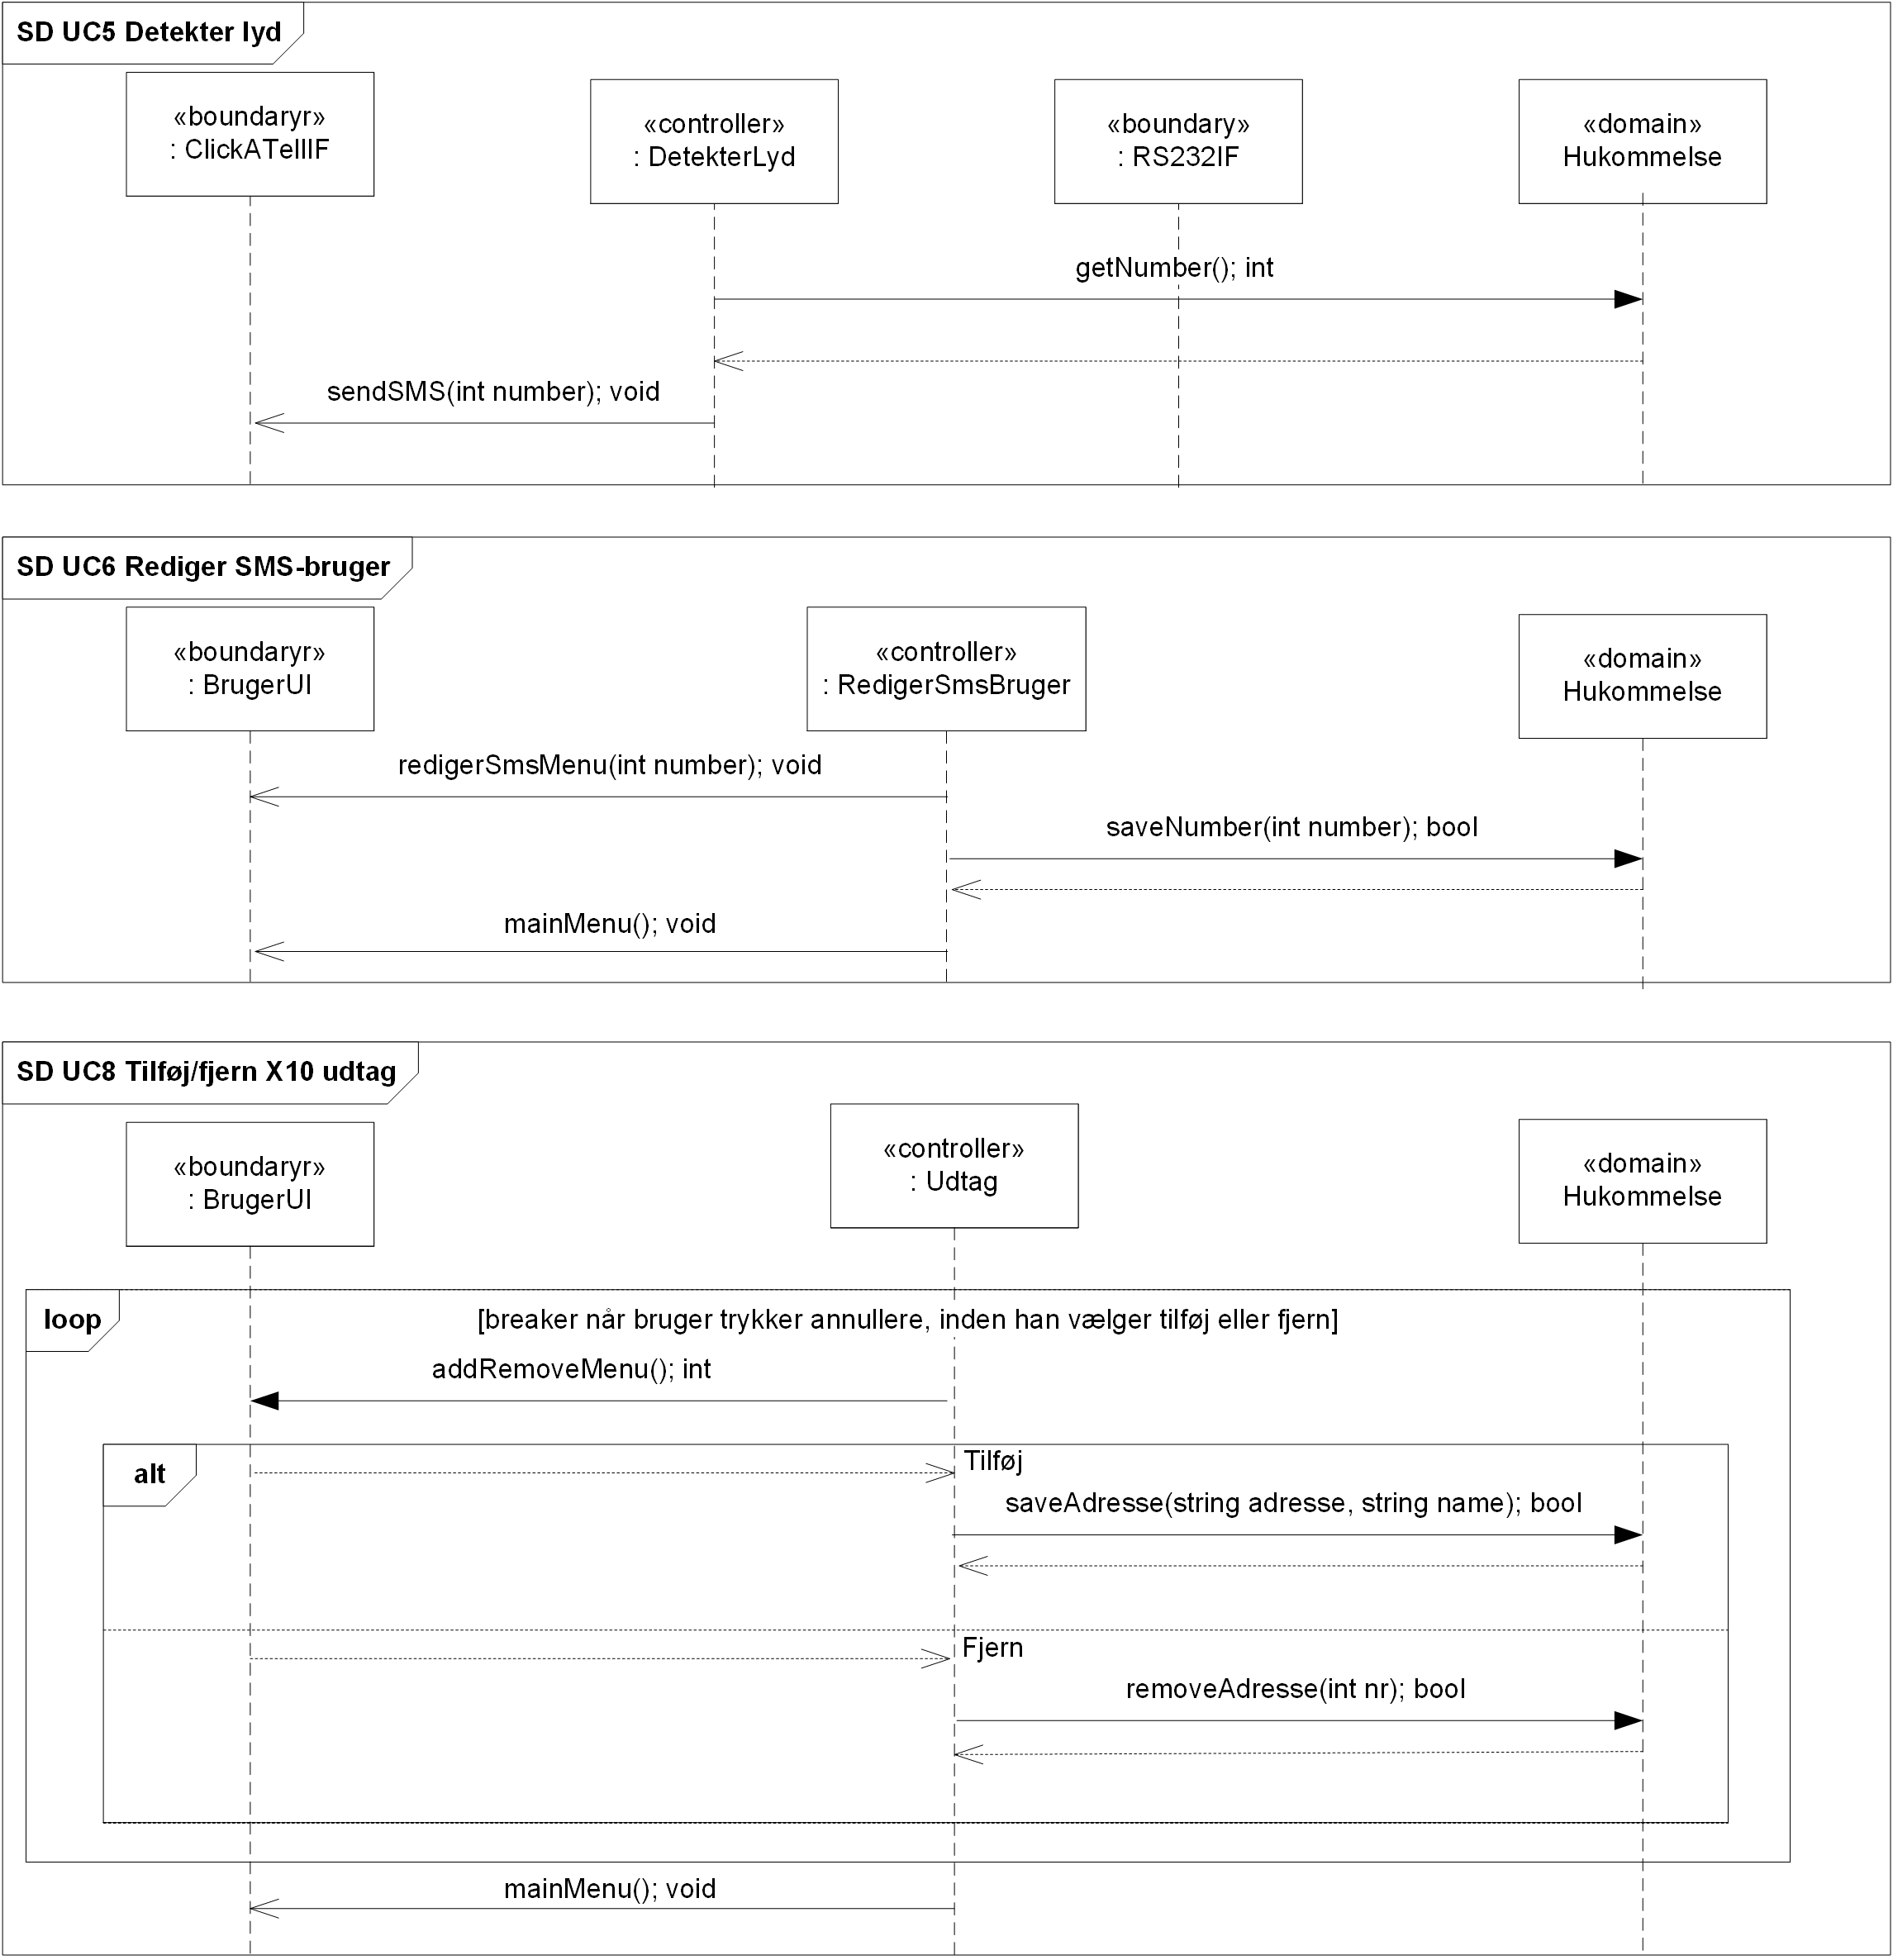
\includegraphics[width=\textwidth]{billeder/uml/PC_SD2}}
     \caption{Use-case 5-8 sekvensdiagram for PC}
     \label{fig:PC_SD2}
\end{figure}
Alle kaldene til controller klasserne kommer fra main.cpp programmet som tager imod bruger inputs i preLogin menuen og mainMenuen. Når mainMenuen er vist så står main.cpp og spørger på read() metoden i RS232IF klassen som tester om den har modtaget data fra STK kittet. Dette gør den for at se om login status har ændret sig eller om der skal sendes en sms til brugeren pga. babyalarmen.\\
Metode navnene i controller klasserne kan ses på næste sidste i klassediagrammet som er lavet på baggrund af Sekvens diagrammerne.

\begin{figure}[!htb]
     {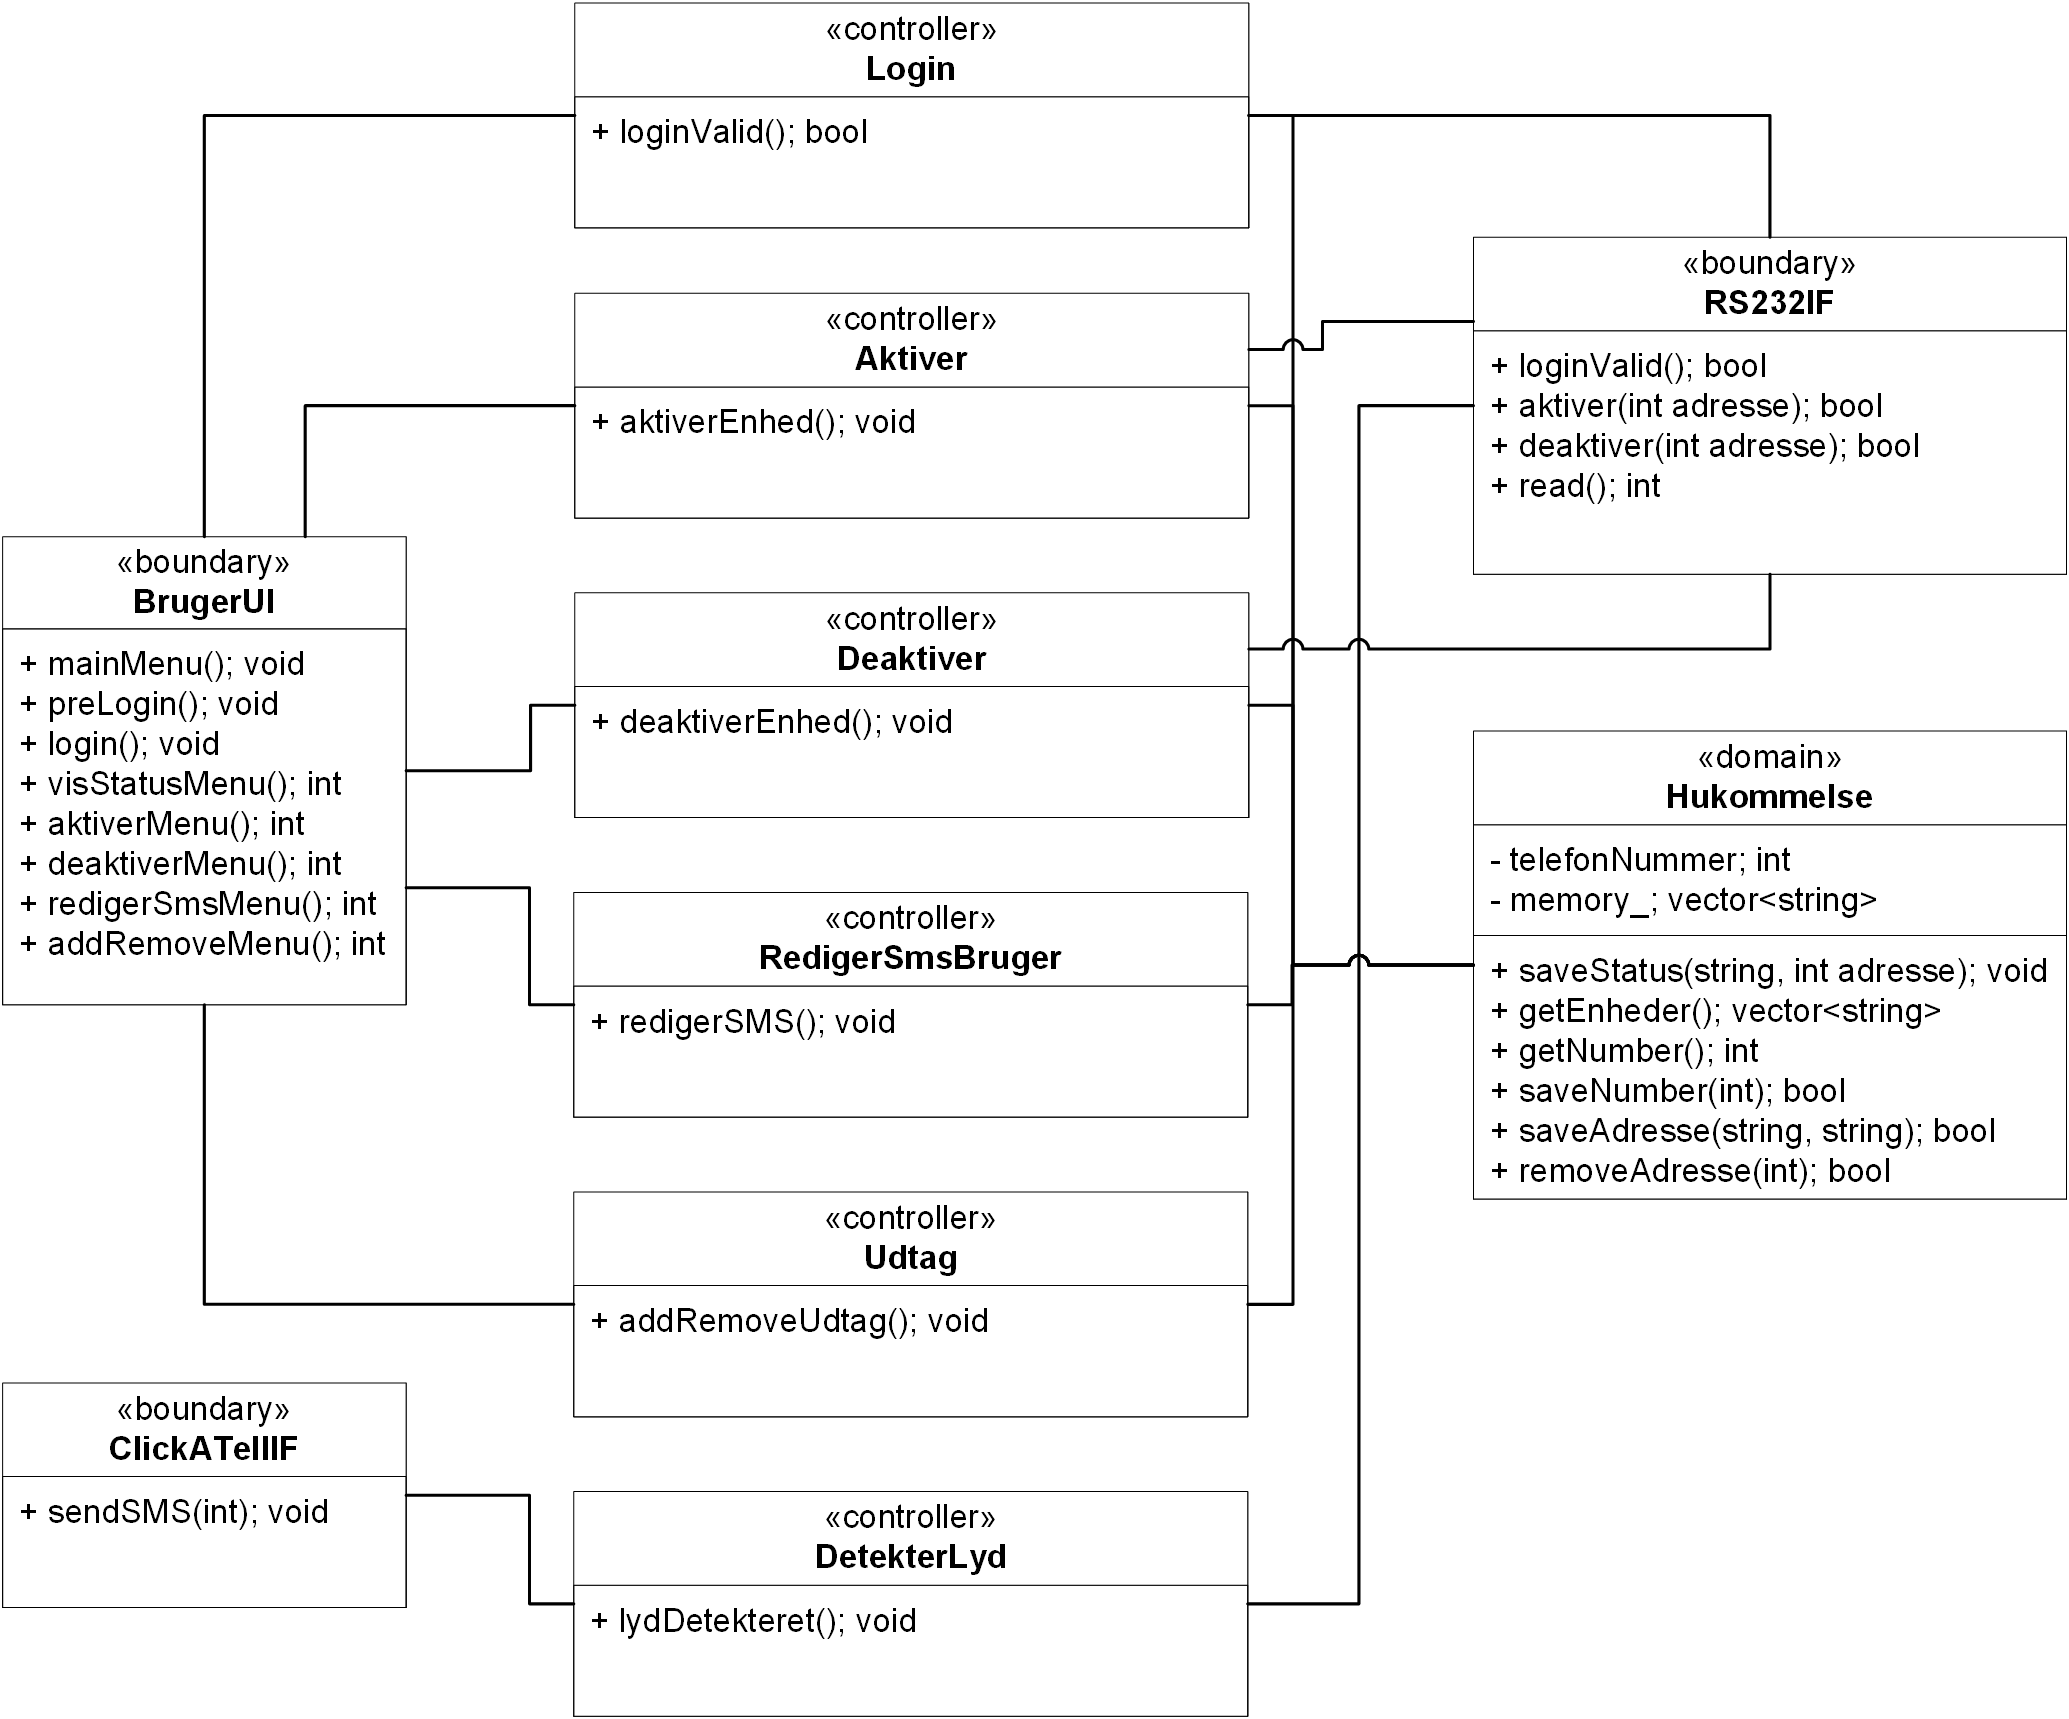
\includegraphics[width=\textwidth]{billeder/uml/PC_Class}}
     \caption{Klassediagram for PC}
     \label{fig:PC_Class}
\end{figure}

\clearpage
\vspace*{30 px}
\begin{figure}[!htb]
     {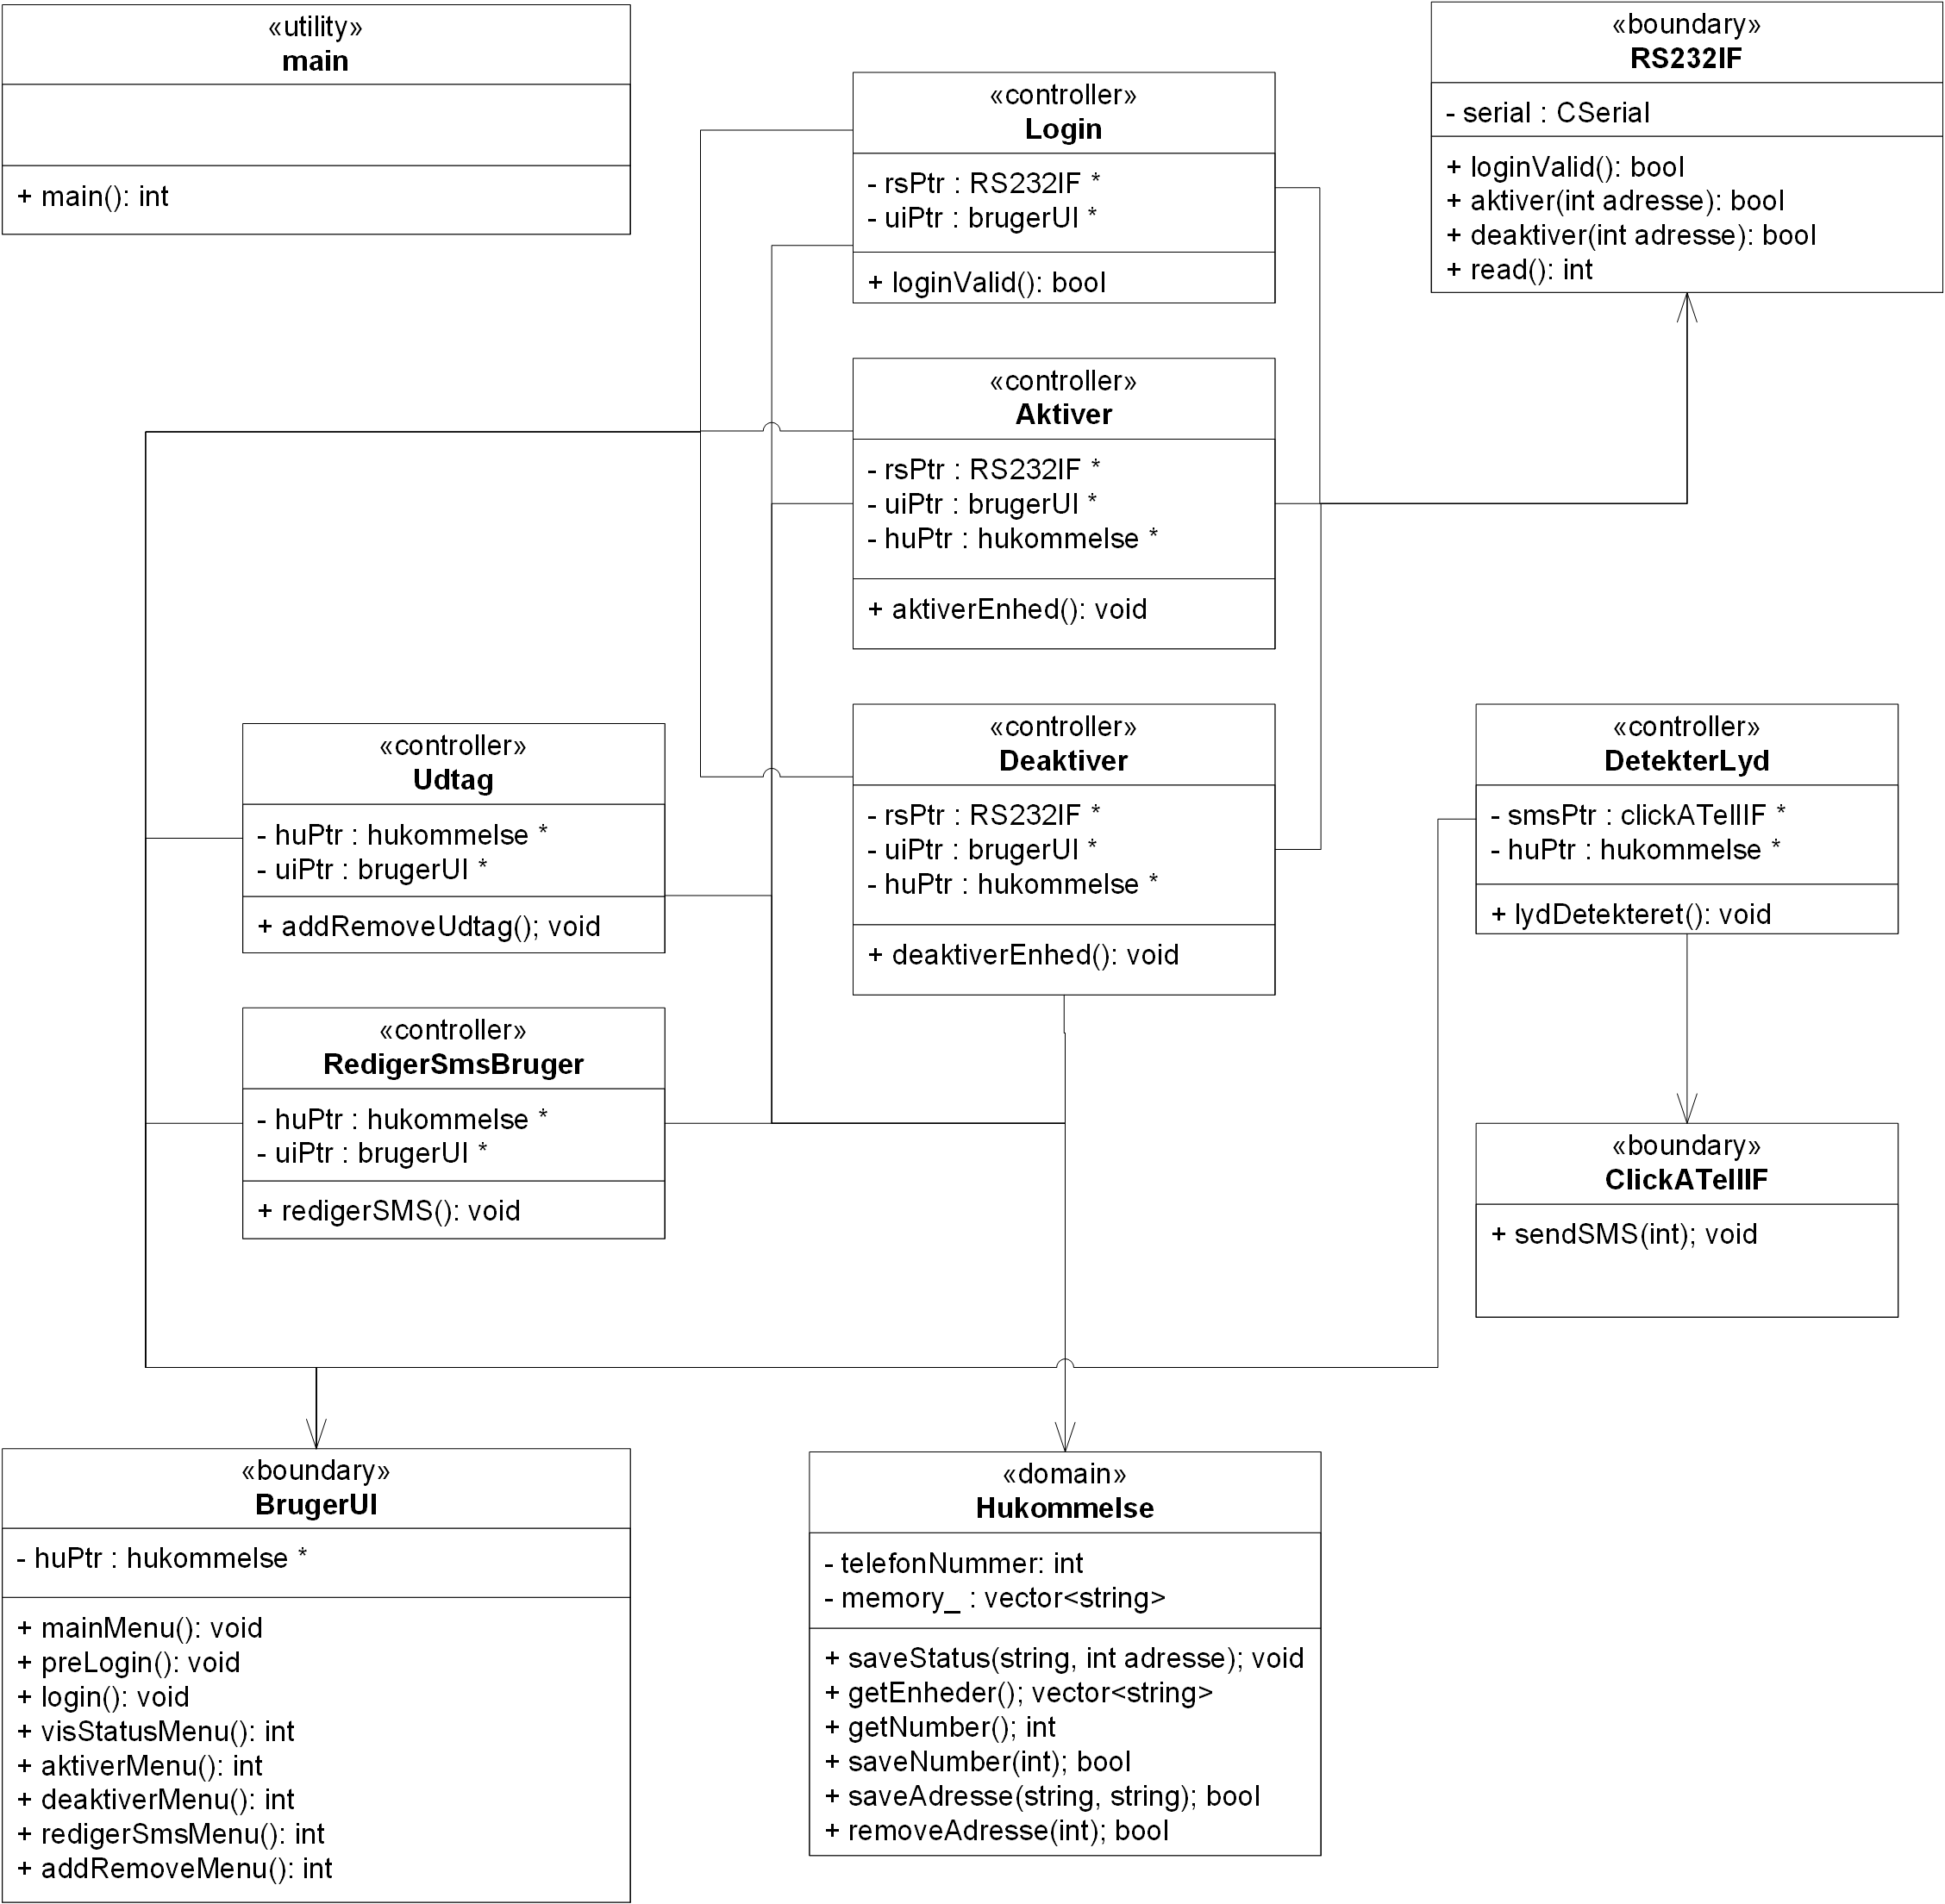
\includegraphics[width=\textwidth]{billeder/uml/PC_Class_static}}
     \caption{Statisk klassediagram for PC}
     \label{fig:PC_Class}
\end{figure}

Main opretter alle objekterne og pointerne til de klasser hvis constructor skal bruge dem. Derudover styre main hvilke controllers der bliver kaldt alt efter bruger input.
%
%\begin{figure}[!htb]
%     \xput[0.471]{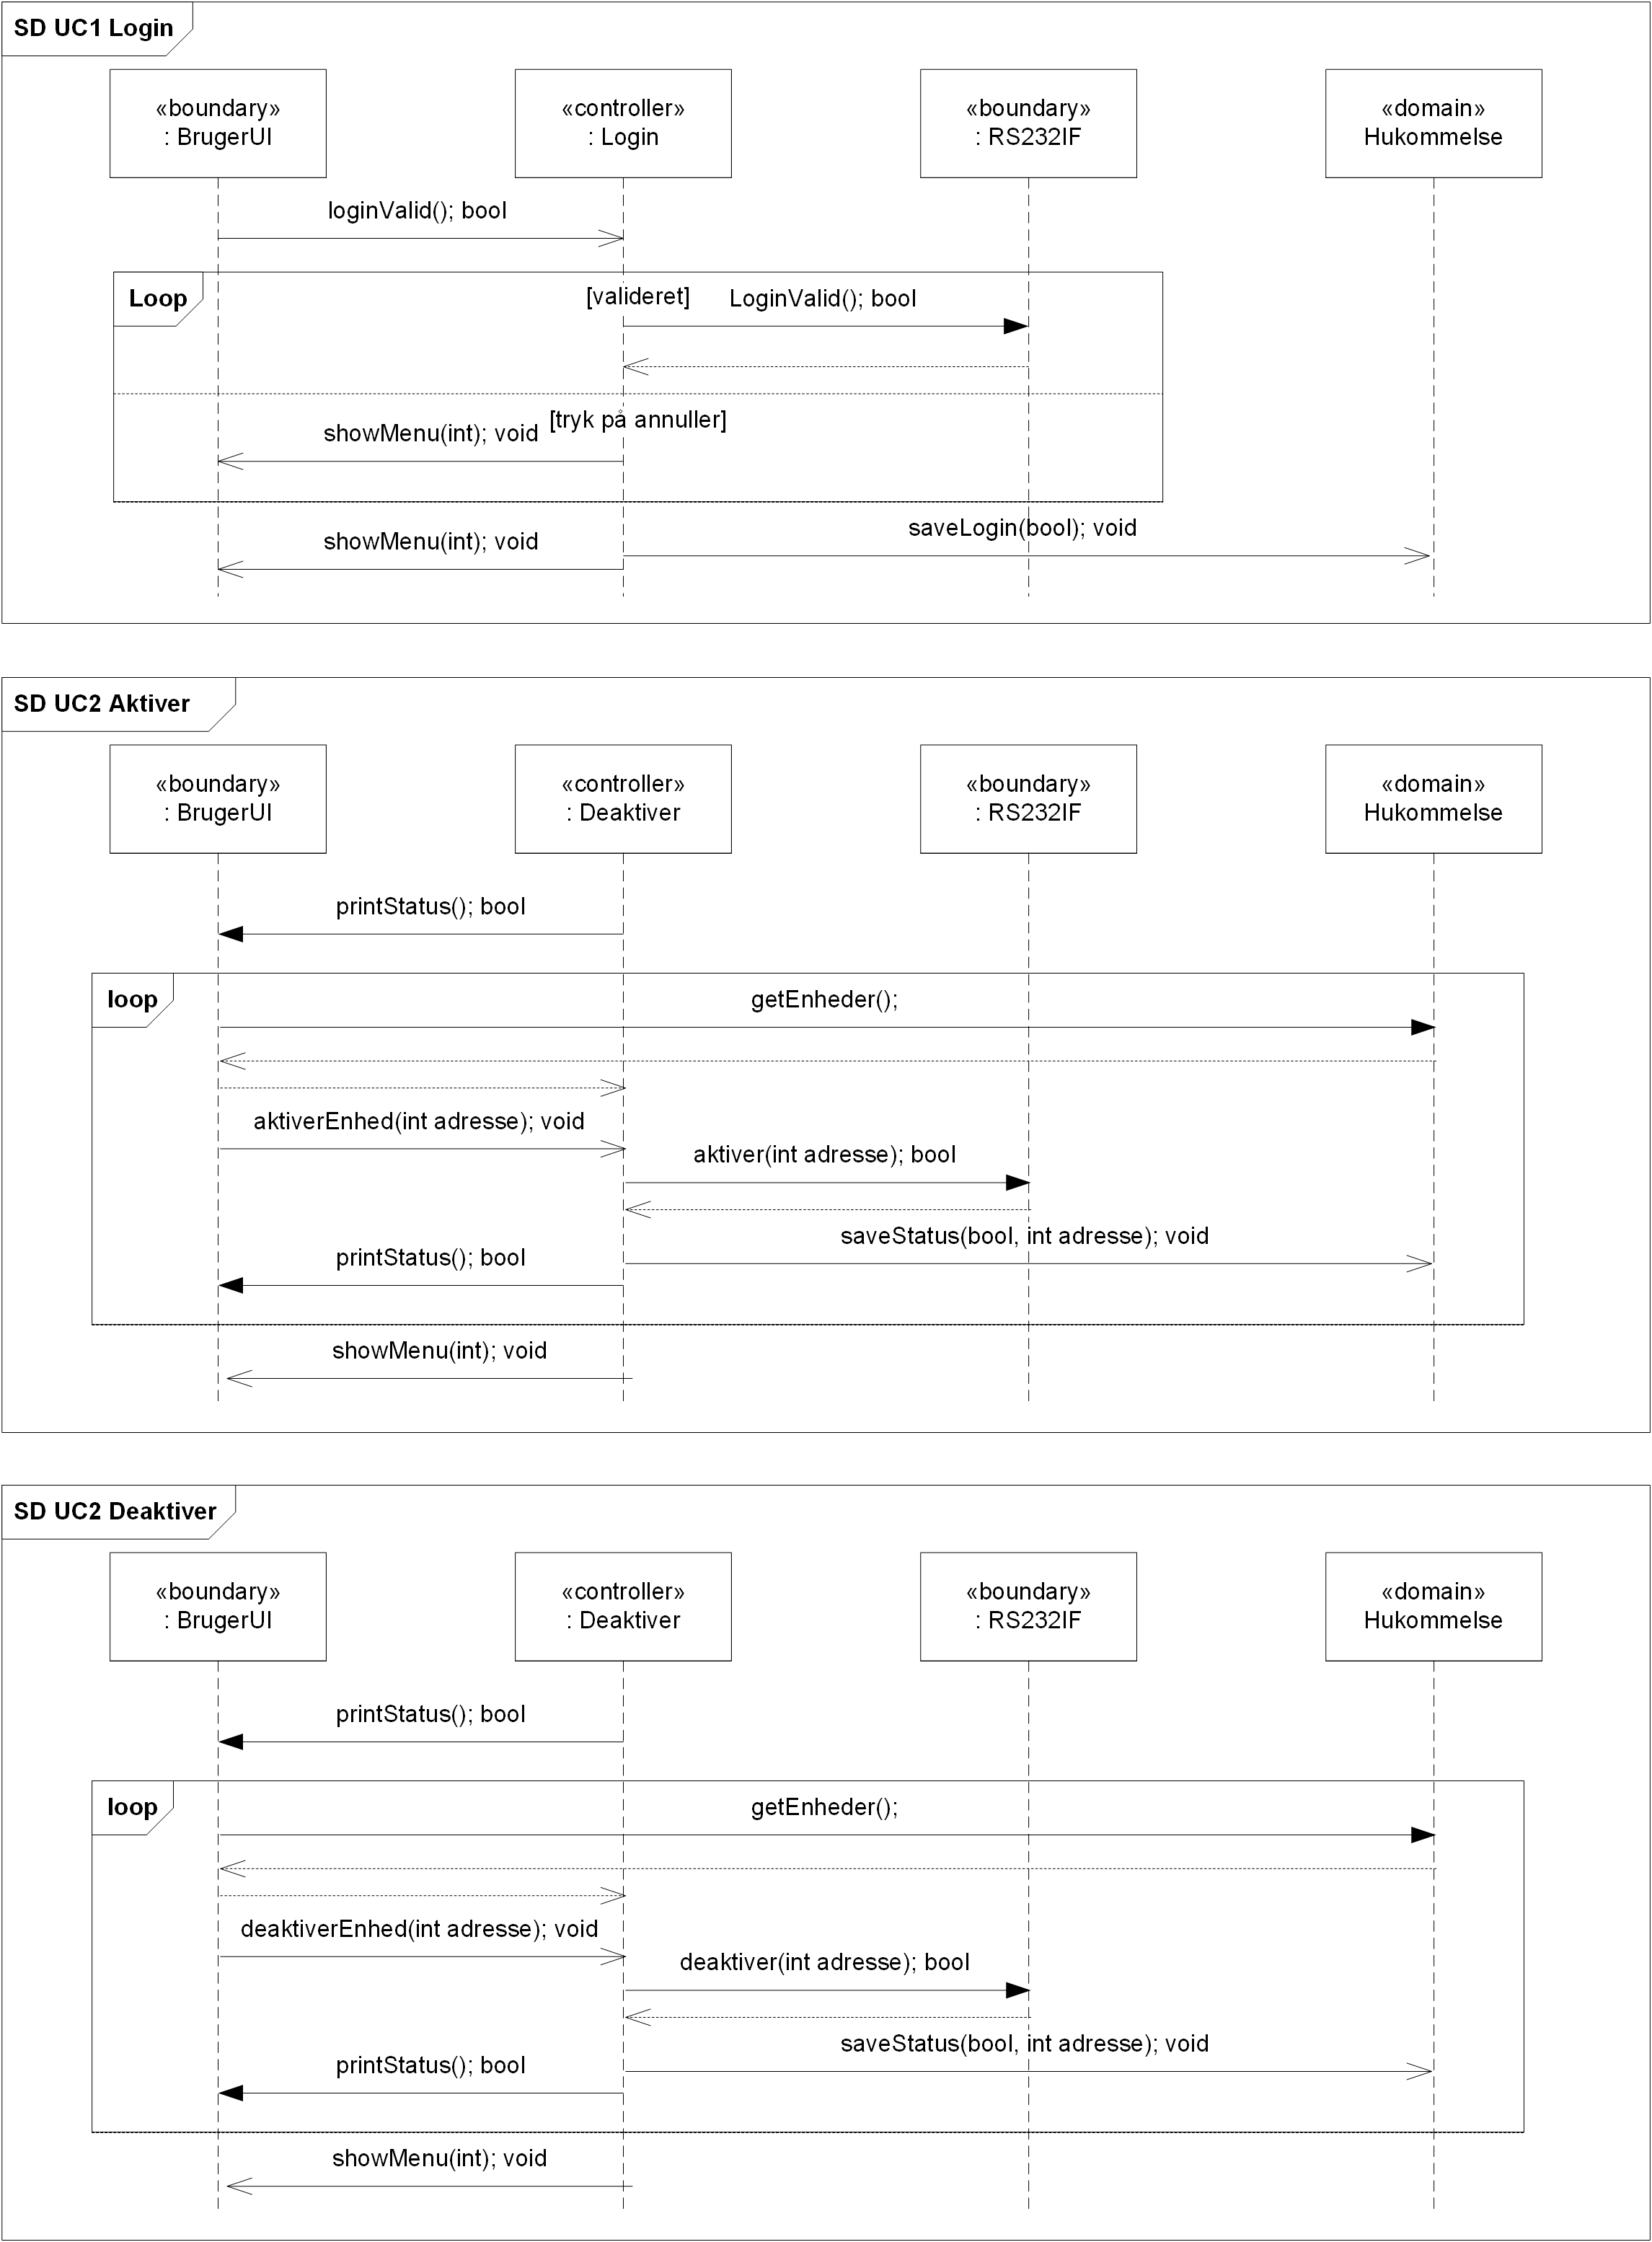
\includegraphics[width=1.32\linewidth]{billeder/uml/PC_SD1}}
%     \caption{Use-case 1-3 sekvensdiagram for PC}
%     \label{fig:PC_SD1}
%\end{figure}
